\documentclass[fontscale=0.38,a0paper]{baposter}

\tracingstats=2

\usepackage{times}
\usepackage{calc}
\usepackage{graphicx}
\usepackage{amsmath}
\usepackage{amssymb}
\usepackage{relsize}
\usepackage{multirow}
\usepackage{bm}
\usepackage{caption}
\usepackage[authoryear,round]{natbib}
\usepackage[hidelinks]{hyperref}

\usepackage{tabularx}
\usepackage{booktabs}

\usepackage{colortbl}

\usepackage{multicol}

%\usepackage{pgfbaselayers}
%\pgfdeclarelayer{background}
%\pgfdeclarelayer{foreground}
%\pgfsetlayers{background,main,foreground}


%\usepackage{tikz}
%\usetikzlibrary{arrows,backgrounds,patterns,matrix,shapes,fit,calc,shadows,plotmarks,decorations.pathmorphing,positioning,trees}

\renewcommand{\familydefault}{\sfdefault}
\usepackage{helvet}
\usepackage{bookman}
\usepackage{palatino}

% My stuff
\newcommand{\R}{\mathbb{R}}
\newcommand{\E}{\mathbb{E}}
\renewcommand{\P}{\mathbb{P}}
\newcommand{\st}{\,\colon\,}
\newcommand{\bone}{\mathbf{1}}
\newcommand{\var}{\mathop{\mbox{Var}}}
\newcommand{\cov}{\mathop{\mbox{cov}}}
\newcommand{\tskit}{{\texttt{tskit}}}
\newcommand{\branch}{\mbox{Branch}} % branch stat
\newcommand{\branchp}{\mbox{Branch}_+} % polarised
\newcommand{\site}{\mbox{Site}} % site stat
\newcommand{\sitep}{\mbox{Site}_+} % polarised
\newcommand{\node}{\mbox{Node}} % node stat
\newcommand{\nodep}{\mbox{Node}_+} % polarised
\newcommand{\given}{\;\vert\;}

\newcommand{\treeseq}{\mathbb{T}} % tree sequence
\newcommand{\iw}{w} % sample (initial) weights
\newcommand{\tiw}{w_\text{total}} % total sample (initial) weights
\newcommand{\nw}{x} % subtree (node) weights
\newcommand{\aw}{{\bar x}} % allele weights


% end my stuff

\selectcolormodel{cmyk}

% \graphicspath{{images/}}

%%%%%%%%%%%%%%%%%%%%%%%%%%%%%%%%%%%%%%%%%%%%%%%%%%%%%%%%%%%%%%%%%%%%%%%%%%%%%%%%
%%%% Some symbols used in the text
%%%%%%%%%%%%%%%%%%%%%%%%%%%%%%%%%%%%%%%%%%%%%%%%%%%%%%%%%%%%%%%%%%%%%%%%%%%%%%%%
%\newcommand{\sub}[2]{\ensuremath{#1_{\textrm{#2}}}}
%\newcommand{\gen}[2]{\ensuremath{\textrm{#1}_{\textrm{#2}}}}


%%%%%%%%%%%%%%%%%%%%%%%%%%%%%%%%%%%%%%%%%%%%%%%%%%%%%%%%%%%%%%%%%%%%%%%%%%%%%%%%
% Multicol Settings
%%%%%%%%%%%%%%%%%%%%%%%%%%%%%%%%%%%%%%%%%%%%%%%%%%%%%%%%%%%%%%%%%%%%%%%%%%%%%%%%
\setlength{\columnsep}{1em}
\setlength{\columnseprule}{0mm} % no vertical line


%%%%%%%%%%%%%%%%%%%%%%%%%%%%%%%%%%%%%%%%%%%%%%%%%%%%%%%%%%%%%%%%%%%%%%%%%%%%%%%%
% Save space in lists. Use this after the opening of the list
%%%%%%%%%%%%%%%%%%%%%%%%%%%%%%%%%%%%%%%%%%%%%%%%%%%%%%%%%%%%%%%%%%%%%%%%%%%%%%%%
\newcommand{\compresslist}{
\setlength{\itemsep}{1pt}
\setlength{\parskip}{0pt}
\setlength{\parsep}{0pt}
}

%%%%%%%%%%%%%%%%%%%%%%%%%%%%%%%%%%%%%%%%%%%%%%%%%%%%%%%%%%%%%%%%%%%%%%%%%%%%%%
%%% Other Macros
%%%%%%%%%%%%%%%%%%%%%%%%%%%%%%%%%%%%%%%%%%%%%%%%%%%%%%%%%%%%%%%%%%%%%%%%%%%%%%
% \renewcommand{\labelenumi}{\alph{enumi})}
% \renewcommand{\theenumi}{\alph{enumi})}
\newcommand{\postercaption}[1]{\begin{minipage}{\linewidth}\center\smaller
  {#1}\end{minipage}}



%%%%%%%%%%%%%%%%%%%%%%%%%%%%%%%%%%%%%%%%%%%%%%%%%%%%%%%%%%%%%%%%%%%%%%%%%%%%%%
%%% Begin of Document
%%%%%%%%%%%%%%%%%%%%%%%%%%%%%%%%%%%%%%%%%%%%%%%%%%%%%%%%%%%%%%%%%%%%%%%%%%%%%%

\begin{document}

%%%%%%%%%%%%%%%%%%%%%%%%%%%%%%%%%%%%%%%%%%%%%%%%%%%%%%%%%%%%%%%%%%%%%%%%%%%%%%
%%% Here starts the poster
%%%---------------------------------------------------------------------------
%%% Format it to your taste with the options
%%%%%%%%%%%%%%%%%%%%%%%%%%%%%%%%%%%%%%%%%%%%%%%%%%%%%%%%%%%%%%%%%%%%%%%%%%%%%%

% Define some colors
\definecolor{silver}{cmyk}{0,0,0,0.3}
\definecolor{black}{cmyk}{0,0,0.0,1.0}
\definecolor{white}{cmyk}{0,0,0.0,0.0}
\definecolor{darkSilver}{cmyk}{0,0,0,0.1}

\definecolor{darkYellow}{cmyk}{0,0,1.0,0.5}
\definecolor{yellow}{cmyk}{0,0,0.9,0.0}
\definecolor{reddishyellow}{cmyk}{0,0.22,1.0,0.0}
\definecolor{lightyellow}{cmyk}{0,0,0.3,0.0}
\definecolor{lighteryellow}{cmyk}{0,0,0.1,0.0}
\definecolor{lightestyellow}{cmyk}{0,0,0.05,0.0}

\definecolor{DavisBlue}{cmyk}{1,0.56,0,0.34}
%    C = 100  M = 56  Y = 0 K = 34


\definecolor{HohenheimBlue}{cmyk}{1,0.5,0,0.45}
\definecolor{HohenheimLightLightBlue}{RGB}{243,250,255}
\definecolor{HohenheimLightBlue}{RGB}{215,221,235}
\definecolor{HohenheimDarkBlue}{RGB}{52,104,152}
\definecolor{darkCyan}{cmyk}{1,1,0,0.5}
\definecolor{cyan}{cmyk}{1,0,0,0.0}
\definecolor{lightcyan}{cmyk}{0.3,0,0,0.0}
\definecolor{lightercyan}{cmyk}{0.1,0,0,0.0}
\definecolor{lightestcyan}{cmyk}{0.05,0,0,0.0}



\typeout{Poster Starts}
%Define custom background
\background{
  \begin{tikzpicture}[remember picture,overlay]%
    \draw (current page.north west)+(-2em,2em) node[anchor=north west] {\includegraphics[height=\textheight]{silhouettes_background}};
  \end{tikzpicture}%
}

\newlength{\leftimgwidth}
\begin{poster}%
  % Poster Options
  {
  % Columns and Column spacing
  columns=3,
  colspacing=1.5em,
  % Background
  % background=user,
  background=shade-tb,
  % Poster header options
  eyecatcher=yes,
  posterheaderheight=0.15\textheight,
  % Format of textbox header
  headerborder=open,
  % headershape=small-rounded,
  headershape=roundedright,
  headershade=shade-tb,
  % headershade=plain,
  headerfont=\Large\textsf, %Sans Serif
  % Format of textbox
  boxborder=small-rounded,
  % boxborder=roundedleft,    
  boxshade=plain,
  linewidth=0.5pt,
  % Color style
  % bgColorOne=lightestcyan,
  % bgColorTwo=lightcyan,
  bgColorOne=white,
  bgColorTwo=white,
  % borderColor=cyan,
  borderColor=black,
  headerColorOne=DavisBlue,
  % headerColorOne=cyan,
  headerColorTwo=black,
  % headerFontColor=black,
  headerFontColor=white,
  % boxColorOne=lightercyan,
  boxColorOne=HohenheimLightLightBlue,
  boxColorTwo=white,
  % Show grid to help with alignment
  grid=no
  % grid=yes
  }
  % Eye Catcher
  {
  \makebox[15em][r]{%
    \begin{minipage}{15em}
       \hfill
       
\includegraphics[width=15em]{tskit_logo} \\
    \end{minipage}
    }
  }
  % Title
  {\sf %Sans Serif
  %\bf% %bold  
  \vspace{0.5em}
     \textbf{\textcolor{DavisBlue}{Spatial models in population genetics}}\vspace{0.5em}}
  % Authors
  {\sf %Sans Serif
    Alison Etheridge${}^\dagger$,
    Tom Kurtz,${}^\S$,
    Ian Letter${}^\dagger$,
    Gilia Patterson$^{\ddagger}$,
    Peter Ralph$^{\ddagger}$,
    \\  \vspace{-1.0mm}
    and Terence Tsui${}^\dagger$.
Code: \url{github.com/petrelharp/probgen-2022-poster}. 
    \\  \vspace{-1.0mm}
    {\small \textit{$\ddagger$ Mathematics and Biology, University of Oregon} }\\ \vspace{-0.5em}
    {\small \textit{$\dagger$ Department of Statistics, University of Oxford} }\\ \vspace{-0.5em}
    {\small \textit{$\S$ Departments of Mathematics and Statistics, University of Wisconsin - Madison}} \\
  }
  % Project logo
  {
    \makebox[15em][r]{%
      \begin{minipage}{12em}
        \hfill
          
\includegraphics[width=10em]{UOSignature-STK-BLK} \\
      \end{minipage}
    }
  }

  % Width of left inset image
%  \setlength{\leftimgwidth}{0.78em+0.0em}

%%%%%%%%%%%%%%%%%%%%%%%%%%%%%%%%%%%%%%%%%%%%%%%%%%%%%%%%%%%%%%%%%%%%%%%%%%%%%%
%%% Now define the boxes that make up the poster
%%%---------------------------------------------------------------------------
%%% Each box has a name and can be placed absolutely or relatively.
%%% The only inconvenience is that you can only specify a relative position 
%%% towards an already declared box. So if you have a box attached to the 
%%% bottom, one to the top and a third one which should be in between, you 
%%% have to specify the top and bottom boxes before you specify the middle 
%%% box.
%%%%%%%%%%%%%%%%%%%%%%%%%%%%%%%%%%%%%%%%%%%%%%%%%%%%%%%%%%%%%%%%%%%%%%%%%%%%%%

%%%%%%%%%%%%%%%%%%%%%%%%%%%%%%%%%%%%%%%%%%%%%%%%%%%%%%%%%%%%%%%%%%%%%%%%%%%%%%
\headerbox{Spatial models}{name=models,column=0,row=0,span=1}{
%%%%%%%%%%%%%%%%%%%%%%%%%%%%%%%%%%%%%%%%%%%%%%%%%%%%%%%%%%%%%%%%%%%%%%%%%%%%%%

    There's lots of ways space can enter a model,
    but the trickiest is through population regulation.
Population dynamics must depend on the size somehow,
or else the population will either die out or blow up,
with certainty (no long-term stability).
To do this, we can have:
\begin{enumerate}
        \compresslist
    \item reproduction rate, $\gamma$,
    \item establishment probability, $r$, or
    \item deathrate, $\mu$,
\end{enumerate}
depend on local population density,
measured using a kernel density estimate
(\texttt{i1.localPopulationDensity( )} in SLiM).

The difference between (1) and (2) is that
"local" means either (1) around the parent,
or (2) around the child (after dispersal).


Other spatial aspects of models are:
\textbf{dispersal} of offspring, and/or
\textbf{mate choice}.


Important quantities:
\begin{itemize}
        \compresslist
    \item $N$: equilibrium population density per unit area
    \item $\sigma$: dispersal distance
    \item $\epsilon$, "interaction distance": width of the kernel used to measure population density
    \item $K = 4 N \pi \epsilon^2$: size of interaction neighborhood
    \item $\mathcal{N}_\text{loc} = 4 N \pi \sigma^2$: Wright's neighborhood size
\end{itemize}

}
%%%%%%%%%%%%%%%%%%%%%%%%%%%%%%%%%%%%%%%%%%%%%%%%%%%%%%%%%%%%%%%%%%%%%%%%%%%%%%


%%%%%%%%%%%%%%%%%%%%%%%%%%%%%%%%%%%%%%%%%%%%%%%%%%%%%%%%%%%%%%%%%%%%%%%%%%%%%%
\headerbox{Debugging your model}{name=debugging,column=0,below=models,span=1}{
%%%%%%%%%%%%%%%%%%%%%%%%%%%%%%%%%%%%%%%%%%%%%%%%%%%%%%%%%%%%%%%%%%%%%%%%%%%%%%


It's easy to get populations that die out or quickly get too big.
Here's a recipe to get what you want:

1. Pick functional forms so that
    $F(x) := r(x) \gamma(x) - \mu(x)$ has
    $F(x) > 0$ for $x < 1$ and $F(x) < 0$ for $x > 1$.

2. Pick a equilibrium density $N$,
   and at local density $u$,
   set establishment probability to $r(u/N)$,
   mean number of offspring to $\gamma(u/N)$,
   and probability of death to $\mu(u/N)$.

3. Ideally you'd be done, but there will be problems:
    for instance, discrete time steps.
    Adjust by multiplying $\mu$ by a constant $\alpha$
    chosen so that a nonspatial population of size $K$
    is stable on average,
    by numerical simulation.

Don't forget to look at plots of $r$, $\gamma$, $\mu$, and $F$,
and your nonspatial population dynamics!

}
%%%%%%%%%%%%%%%%%%%%%%%%%%%%%%%%%%%%%%%%%%%%%%%%%%%%%%%%%%%%%%%%%%%%%%%%%%%%%%

%%%%%%%%%%%%%%%%%%%%%%%%%%%%%%%%%%%%%%%%%%%%%%%%%%%%%%%%%%%%%%%%%%%%%%%%%%%%%%
\headerbox{A note of caution}{name=caution,column=0,below=debugging,span=1}{
%%%%%%%%%%%%%%%%%%%%%%%%%%%%%%%%%%%%%%%%%%%%%%%%%%%%%%%%%%%%%%%%%%%%%%%%%%%%%%

    Here are screenshots from a straightforward spatial model, with
    death rate $\mu=0.3$ per generation, establishment probability of $r=0.7$,
    Gaussian dispersal with SD $\sigma$, 
    local density measured in a circle of radius $\epsilon=1$,
    and reproduction rate equal to 
        $$ \gamma = \frac{\lambda}{1 + \text{(local density)}/K} $$
    with $K=2$ and $\lambda=3$.
SLiM code on github (URL above).

Left: $\sigma = 3$. Right: $\sigma=0.2$.

    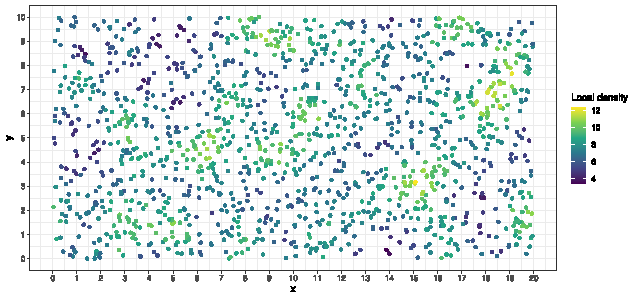
\includegraphics[width=0.5\textwidth]{figs/gilia_high_sigma}
    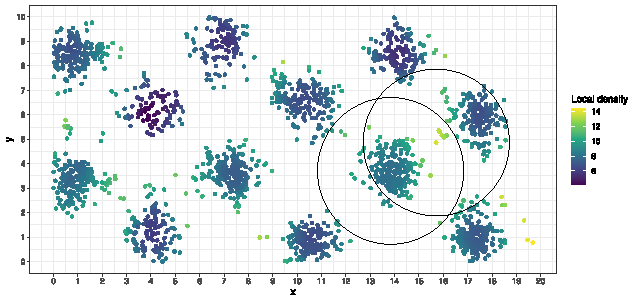
\includegraphics[width=0.5\textwidth]{figs/gilia_low_sigma}

What's going on?
Imagine interactions are mediated by depleetion of resources.
The clumping pattern on the right is stable because areas between clumps
have resources removed by more than one clump.
There is always this tendency in a model,
but we only see it if
dispersal ($\sigma$) is less than the interaction distance ($\epsilon$).
See section 16.10 in the SLiM manual,
or
\citet{sasaki1997clumped}.
\emph{Note:} if you actually \emph{want} clumps,
you probably want an Allee effect,
not this.


}
%%%%%%%%%%%%%%%%%%%%%%%%%%%%%%%%%%%%%%%%%%%%%%%%%%%%%%%%%%%%%%%%%%%%%%%%%%%%%%


%%%%%%%%%%%%%%%%%%%%%%%%%%%%%%%%%%%%%%%%%%%%%%%%%%%%%%%%%%%%%%%%%%%%%%%%%%%%%%
\headerbox{}{name=scales,column=1,row=0,span=1}{
%%%%%%%%%%%%%%%%%%%%%%%%%%%%%%%%%%%%%%%%%%%%%%%%%%%%%%%%%%%%%%%%%%%%%%%%%%%%%%

    Two sorts of spatial relations:
    offspring disperse (left)
    and nearby individuals interact (right),
    affecting each other's fitness:

    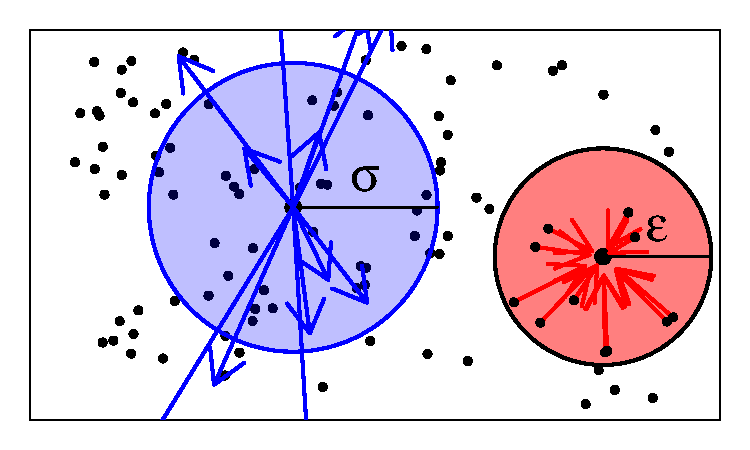
\includegraphics[width=\textwidth]{figs/scales_diagram}

}
%%%%%%%%%%%%%%%%%%%%%%%%%%%%%%%%%%%%%%%%%%%%%%%%%%%%%%%%%%%%%%%%%%%%%%%%%%%%%%


%%%%%%%%%%%%%%%%%%%%%%%%%%%%%%%%%%%%%%%%%%%%%%%%%%%%%%%%%%%%%%%%%%%%%%%%%%%%%%
\headerbox{A mathematical model}{name=notation,column=1,below=scales,span=1}{
%%%%%%%%%%%%%%%%%%%%%%%%%%%%%%%%%%%%%%%%%%%%%%%%%%%%%%%%%%%%%%%%%%%%%%%%%%%%%%

    We're working on a formal description of the scaling limits
    of models like this,
    along with the model's lineages.

\begin{itemize}
        \compresslist
    \item $N$: scaling factor for density
    \item $\eta_t$: point measure with mass $1/N$ for each individual
    \item $\gamma(x, \eta_t)$: per capita birth rate at $x$
    \item $q(x, dy)$: probability a juvenile disperses to $y$
    \item $r(y, \eta_t)$: juvenile establishment probability at $y$
    \item $\mu(x, \eta_t)$: death rate at $x$
\end{itemize}


The (forwards) *dispersal distance* is:
$$ \sigma^2 = \int |y-x|^2 q(x, dy) .$$



Birth, establishment, and establishment rates
depend on local population densities (like \citet{bolker1997using}):

\begin{itemize}
        \compresslist
    \item $p_\epsilon$: the heat kernel at time $\epsilon^2$
    \item $p_\epsilon * \eta_t(x)$: "local" population density at $x$
    \item $\epsilon$: interaction distance
\end{itemize}


}
%%%%%%%%%%%%%%%%%%%%%%%%%%%%%%%%%%%%%%%%%%%%%%%%%%%%%%%%%%%%%%%%%%%%%%%%%%%%%%


%%%%%%%%%%%%%%%%%%%%%%%%%%%%%%%%%%%%%%%%%%%%%%%%%%%%%%%%%%%%%%%%%%%%%%%%%%%%%%
\headerbox{Scaling limits}{name=limits,column=1,below=notation,span=1}{
%%%%%%%%%%%%%%%%%%%%%%%%%%%%%%%%%%%%%%%%%%%%%%%%%%%%%%%%%%%%%%%%%%%%%%%%%%%%%%

We rescale
$$ N \to \infty \qquad \text{(local density)}$$
and 
$$ \theta \to \infty \qquad \text{(time scaling)} .$$
To retain space:
$$ \sigma \propto \frac{1}{\sqrt{\theta}} \qquad \text{(dispersal distance)}, $$
and to retain temporal dynamics:
$$\begin{aligned}
&\theta \left(r_\theta(x) \gamma_\theta(x) - \mu_\theta(x) \right) \to F(x) \\
&\qquad\qquad \text{(net per capita replacement)} 
\end{aligned}$$

The limit, $\Xi$, ``solves this PDE'':
$$
    \dot \Xi = r \Delta(\gamma \Xi) + F \Xi 
$$
\ldots but recall that the coefficients are "nonlocal": 
$r$ may be a function of $p_\epsilon * \Xi$.

}
%%%%%%%%%%%%%%%%%%%%%%%%%%%%%%%%%%%%%%%%%%%%%%%%%%%%%%%%%%%%%%%%%%%%%%%%%%%%%%

%%%%%%%%%%%%%%%%%%%%%%%%%%%%%%%%%%%%%%%%%%%%%%%%%%%%%%%%%%%%%%%%%%%%%%%%%%%%%%
\headerbox{The governing equation(s)}{name=mean,column=1,below=limits,span=1}{
%%%%%%%%%%%%%%%%%%%%%%%%%%%%%%%%%%%%%%%%%%%%%%%%%%%%%%%%%%%%%%%%%%%%%%%%%%%%%%

The population $\eta$,
encoded by putting mass $1/N$ on each individual,
changes like
$$\begin{aligned}
    & \frac{1}{N} \times N \eta(y) \gamma(y, \eta) \; \hphantom{q(y, dx)} &\qquad &\text{(birth at $y$)} \\
    & \hphantom{\frac{1}{N}} \int \; \hphantom{N \eta(y) \gamma(y, \eta)} \; q(y, dx) r(x, \eta) &\qquad &\text{(dispersal to $x$)}
    \\
    & {} - \frac{1}{N} \times N \eta (x) \mu(x, \eta)  & \qquad &\text{(death)}
\end{aligned}$$
Suppose also the population measure converges,
$\eta \to \Xi$ as $\theta, N \to \infty$.
Then
$$\begin{aligned}
    &
    \lim_{t \searrow 0} \frac{1}{t}
        \left. \mathbb{E} \left[ \int f(x) \eta_{t}(dx) - \int f(x) \eta_0(dx) \;|\; \eta_0 = \eta \right] \right\vert_{t=0} \\
    &\qquad
    \to
        \int \left\{\vphantom{\int}
            \gamma(x, \Xi) \Delta\left(
                    f(\cdot) r(\cdot, \Xi)
                \right)\!(x)
    \right. \\ &\qquad \qquad \qquad \left. \vphantom{\int}
        + f(x) F(x, \Xi) 
    \right\} \Xi(dx) .
\end{aligned}$$

}
%%%%%%%%%%%%%%%%%%%%%%%%%%%%%%%%%%%%%%%%%%%%%%%%%%%%%%%%%%%%%%%%%%%%%%%%%%%%%%


%%%%%%%%%%%%%%%%%%%%%%%%%%%%%%%%%%%%%%%%%%%%%%%%%%%%%%%%%%%%%%%%%%%%%%%%%%%%%%
\headerbox{Superprocess limit and $\mathcal{N}_\text{loc}$}{name=super,column=1,below=mean,span=1}{
%%%%%%%%%%%%%%%%%%%%%%%%%%%%%%%%%%%%%%%%%%%%%%%%%%%%%%%%%%%%%%%%%%%%%%%%%%%%%%

The variance per unit time of $\int f(x) \eta_t(dx)$
is proportional to $1/N$.
So, quadratic variation of the limit is nonzero if
$$ \frac{N}{\theta} \to \rho, $$
for some $\rho > 0$.
Since $\sigma = 1/\sqrt{\theta}$,
Wright's neighborhood size is:
$$\begin{aligned}
    \mathcal{N}_\text{loc}
    &\propto N \sigma^d  \\
    &= \rho \qquad \text{in } d=2.
\end{aligned}$$

}
%%%%%%%%%%%%%%%%%%%%%%%%%%%%%%%%%%%%%%%%%%%%%%%%%%%%%%%%%%%%%%%%%%%%%%%%%%%%%%


%%%%%%%%%%%%%%%%%%%%%%%%%%%%%%%%%%%%%%%%%%%%%%%%%%%%%%%%%%%%%%%%%%%%%%%%%%%%%%
\headerbox{Deterministic limit: $\theta/N \to 0$}{name=det,column=2,row=0,span=1}{
%%%%%%%%%%%%%%%%%%%%%%%%%%%%%%%%%%%%%%%%%%%%%%%%%%%%%%%%%%%%%%%%%%%%%%%%%%%%%%

If the limiting measure has density $\Xi_t(x) dx$,
then it's a weak solution to
$$\begin{aligned}
    \frac{d}{dt} \Xi_t(x)
    &=
        r(x, \Xi) \Delta\left(
                \gamma(\cdot, \Xi_t) \Xi_t(\cdot)
            \right)(x)
        + F(x, \Xi_t) \Xi_t(x) .
\end{aligned}$$

i.e.,
$$\begin{aligned}
    \dot \Xi = r \Delta\left( \gamma \Xi \right) + F \Xi .
\end{aligned}$$
This is an integro-differential equation --
we can take the limit as $\epsilon \to 0$
in certain cases to get a PDE.

}
%%%%%%%%%%%%%%%%%%%%%%%%%%%%%%%%%%%%%%%%%%%%%%%%%%%%%%%%%%%%%%%%%%%%%%%%%%%%%%




%%%%%%%%%%%%%%%%%%%%%%%%%%%%%%%%%%%%%%%%%%%%%%%%%%%%%%%%%%%%%%%%%%%%%%%%%%%%%%
\headerbox{Lineages}{name=lineages,column=2,below=det,span=1}{
%%%%%%%%%%%%%%%%%%%%%%%%%%%%%%%%%%%%%%%%%%%%%%%%%%%%%%%%%%%%%%%%%%%%%%%%%%%%%%

Thanks to a lookdown construction,
following \citet{kurtz2011poisson} and \citet{etheridge2019genealogical},
we can take the limit
while formally retaining lineages.

If a deterministic, local limit holds,
with dispersal $N(m, \sigma^2 I)$,
lineages should move in a stationary population density $n(x) = d\Xi/dx$ as
$$\begin{aligned}
    dL_t = r(L_t) \gamma(L_t) \left\{
            \left(
                2\sigma^2 \nabla \log(n\gamma)(L_t)  - m
            \right) dt
            + \sigma dB_t \right\} .
\end{aligned}$$

i.e., as Brownian motion run at speed $\sigma r(y) \gamma(y)$
in the potential
$$\begin{aligned}
    n(y) \gamma(y) e^{-my/(2\sigma^2)} ,
\end{aligned}$$
... which has stationary distribution
$$\begin{aligned}
    \frac{n(y)}{r(y)} e^{-my/(2\sigma^2)} .
\end{aligned}$$

\textbf{Consequence:} if there is a bias $m$ in migration
then \textbf{genetic diversity is independent of range width},
if it is wider than $\sigma^2 / m$.

}
%%%%%%%%%%%%%%%%%%%%%%%%%%%%%%%%%%%%%%%%%%%%%%%%%%%%%%%%%%%%%%%%%%%%%%%%%%%%%%


%%%%%%%%%%%%%%%%%%%%%%%%%%%%%%%%%%%%%%%%%%%%%%%%%%%%%%%%%%%%%%%%%%%%%%%%%%%%%%
\headerbox{Example: the Porus Medium Equation}{name=pme,column=2,below=lineages,span=1}{
%%%%%%%%%%%%%%%%%%%%%%%%%%%%%%%%%%%%%%%%%%%%%%%%%%%%%%%%%%%%%%%%%%%%%%%%%%%%%%


If we take $r = 1$ and
$$\begin{aligned}
    \gamma(x) &= n(x) \\
    \mu(x) &= (1 + 1/\theta) n(x) - 1/\theta ,
\end{aligned}$$
then the PDE we get is
$$
    \partial_t n_t(x)
    =
    \partial_x^2 n_t(x)^2
    +
    n_t(x)(1 - n_t(x))  \qquad \text{(PME)} .
$$

This has the traveling wave solution
$$\begin{aligned}
    n_t(x) = \left( 1 - \exp\left( \frac{1}{2} (x - t) \right)\right)_+ .
\end{aligned}$$

Population density in simulation, and a numerical solution:

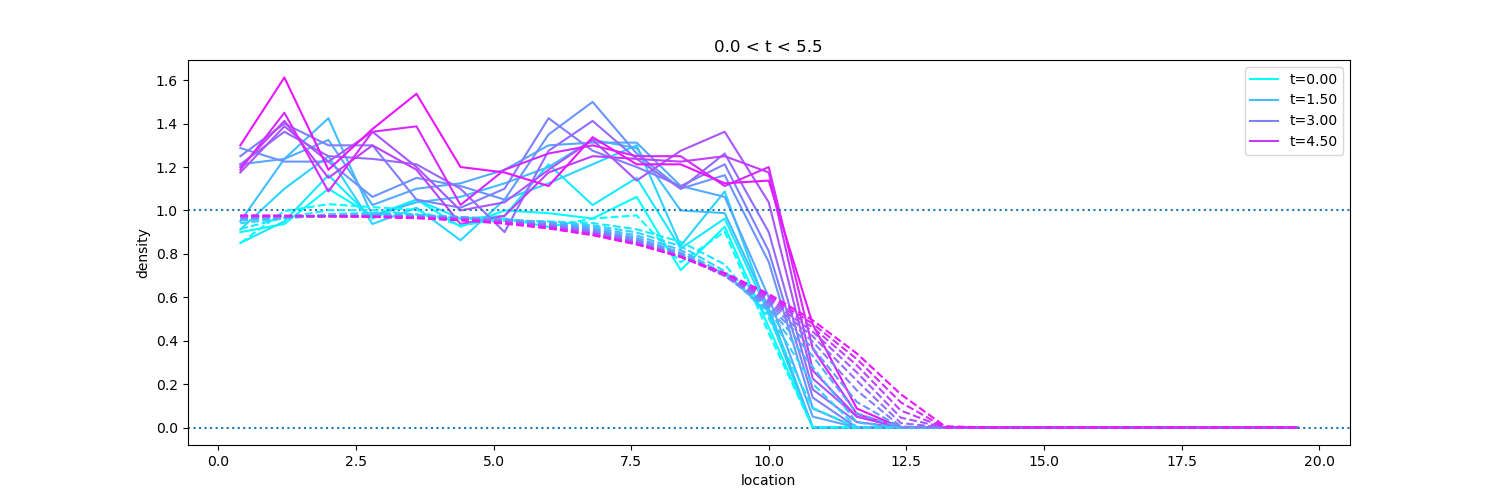
\includegraphics[width=\textwidth]{figs/pme_2439015511154.first_steps.png}

A lineage in the stationary frame has generator
$$\begin{aligned}
    \phi 
    &\mapsto 
    \left(1 - e^{x/2}\right) \phi_{xx}
            + \left(1 - 2 e^{x/2}\right) \phi_x \qquad \text{on } x < 0,
\end{aligned}$$
which has stationary distribution 
$$\begin{aligned}
    \pi(x) \propto e^x \left(1 - e^{x/2}\right)
\end{aligned}$$
for $x < 0$.
This is \emph{different} than the Fisher-KPP behavior!

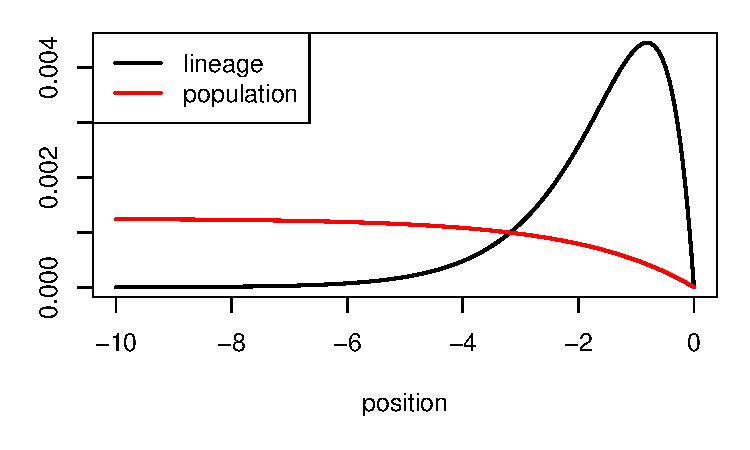
\includegraphics[width=\textwidth]{figs/pme_dists}

}
%%%%%%%%%%%%%%%%%%%%%%%%%%%%%%%%%%%%%%%%%%%%%%%%%%%%%%%%%%%%%%%%%%%%%%%%%%%%%%



%%%%%%%%%%%%%%%%%%%%%%%%%%%%%%%%%%%%%%%%%%%%%%%%%%%%%%%%%%%%%%%%%%%%%%%%%%%%%%
\headerbox{References}{name=refs,column=0,above=bottom}{
%%%%%%%%%%%%%%%%%%%%%%%%%%%%%%%%%%%%%%%%%%%%%%%%%%%%%%%%%%%%%%%%%%%%%%%%%%%%%%
  % \scriptsize
  \renewcommand{\section}[2]{\vskip 0.0em}
  \bibliographystyle{abbrvnat}
  \setlength{\bibsep}{0.0pt}

    Simulations with SLiM (https://messerlab.org/SLiM)
    and msprime
    and tskit (https://tskit.dev)

  \bibliography{refs}
}
%%%%%%%%%%%%%%%%%%%%%%%%%%%%%%%%%%%%%%%%%%%%%%%%%%%%%%%%%%%%%%%%%%%%%%%%%%%%%%


\end{poster}%
\end{document}
